\begin{frame}{Graph Specifications}
% Abstract Refinement Types, Vazou \textit{et al.}, ESOP '13.

Check properties of the vertices and edges affected by the mutation against
defined specifications, for example:

\begin{figure}
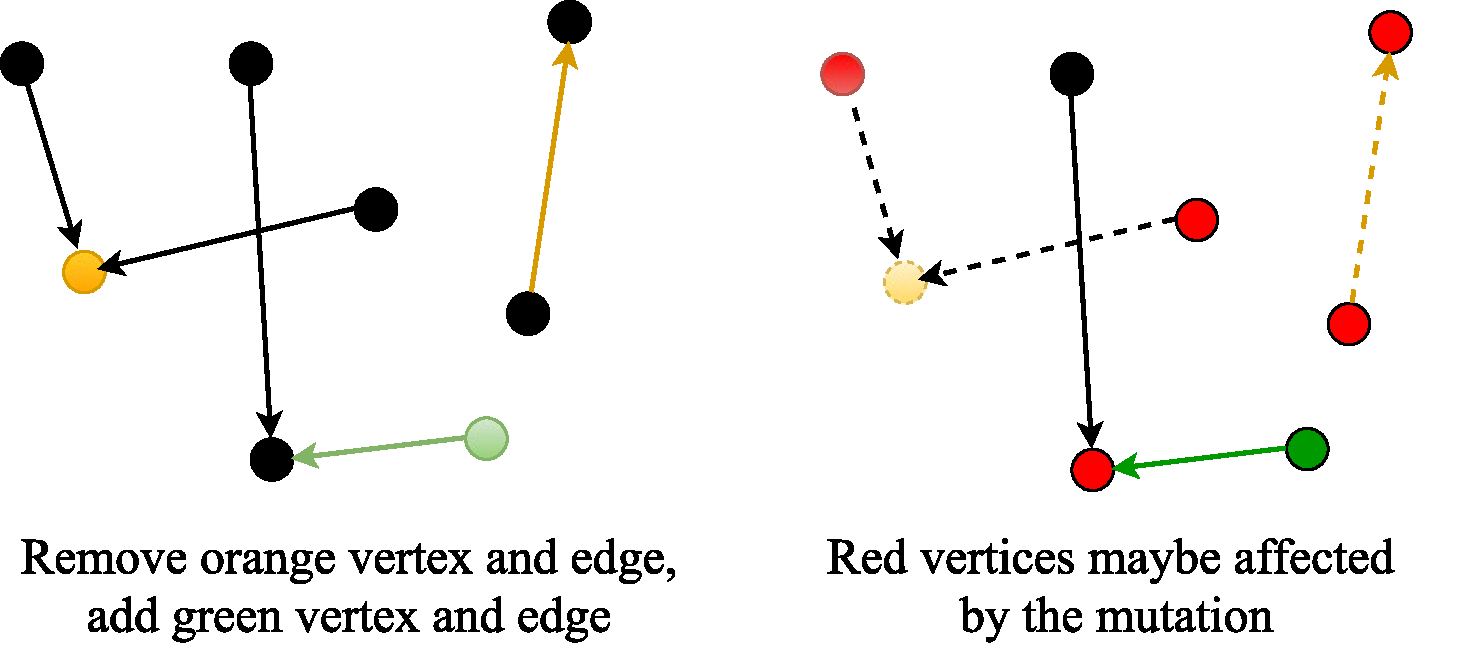
\includegraphics[width=0.8\linewidth]{figures/fig-specification1.pdf}
\end{figure}

Use assertions to check the correctness of mutations.

\begin{itemize}
  \item Maximum in-degree < 2
\end{itemize}

\end{frame}


\begin{frame}
K-clustering problem:
\begin{itemize}
  \item Maximum of 1 cluster node connected.  
\end{itemize}

Restrictions:\\
  Lack of global information, specification may not be able to be on the
  global level.
  
  e.g. checking that the edges being added indeed minimizes the Euclidean
  distance may not be possible as it needs information from different vertices.
\end{frame}

% \begin{frame}
% \begin{figure}
% 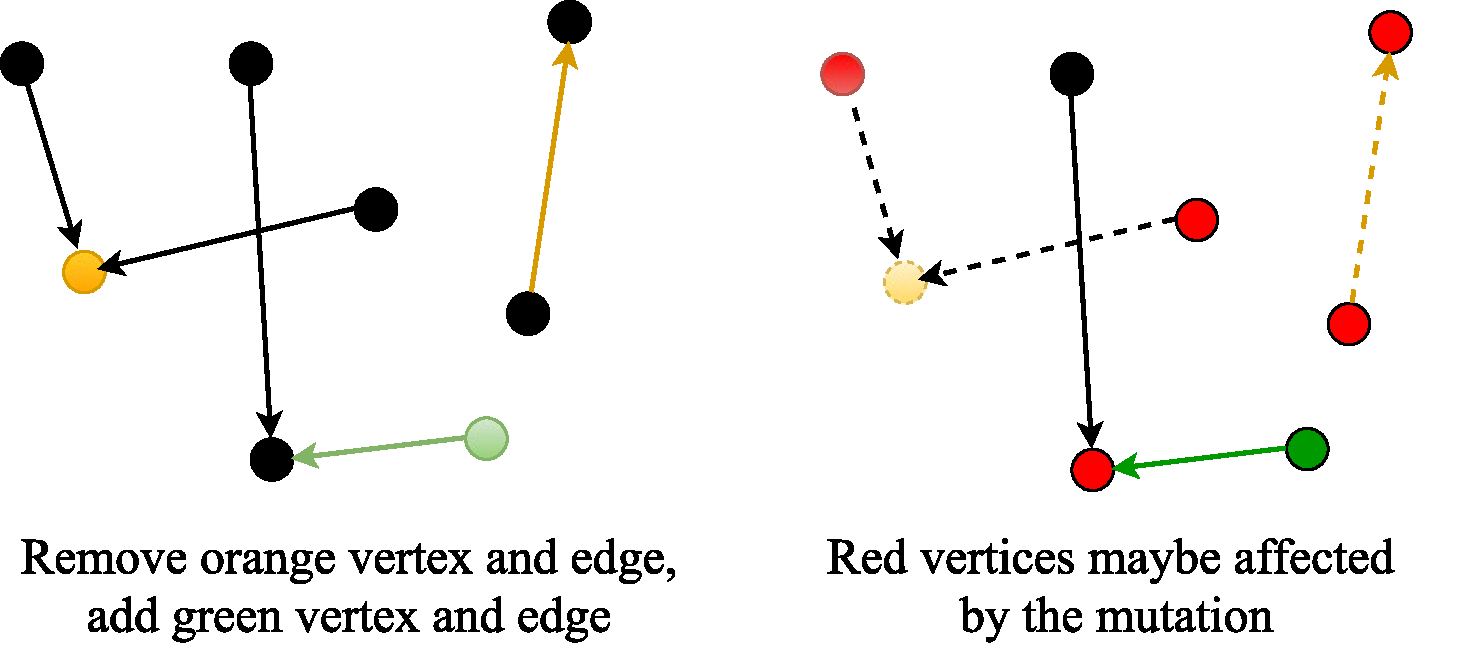
\includegraphics[width=0.8\linewidth]{figures/fig-specification1.pdf}
% \end{figure}
% \end{frame}